\documentclass{article}

\usepackage{fancyhdr}
\usepackage{ragged2e}
\usepackage{graphicx}
\usepackage{caption}
\usepackage{geometry}
\usepackage{amsmath}
\usepackage{rotating}

\usepackage{listings}
\usepackage{color}

\definecolor{dkgreen}{rgb}{0,0.6,0}
\definecolor{gray}{rgb}{0.5,0.5,0.5}
\definecolor{mauve}{rgb}{0.58,0,0.82}

\lstset{frame=tb,
  language=Java,
  aboveskip=3mm,
  belowskip=3mm,
  showstringspaces=false,
  columns=flexible,
  basicstyle={\small\ttfamily},
  numbers=none,
  numberstyle=\tiny\color{gray},
  keywordstyle=\color{blue},
  commentstyle=\color{dkgreen},
  stringstyle=\color{mauve},
  breaklines=true,
  breakatwhitespace=true,
  tabsize=4
}

\setcounter{secnumdepth}{1}

\usepackage{chngcntr}
\counterwithin{figure}{section}

\renewcommand*{\thepage}{C\arabic{page}}

\pagestyle{fancy}
\lhead{ACME Robotics}
\chead{\#8367}
\rhead{\ifcontents Contents \else Week \thesection \fi}

\newif\ifcontents
\contentstrue

\makeatletter
\renewcommand{\@seccntformat}[1]{}
\makeatother

\begin{document}\contentsfalse

\subsection{Design of The Deployment Mechanism}
%! Making marker deployer.
Shawn and Ben worked on revising and iterating the marker deployment mechanism. They discussed the best way to easily drop the marker and came up with a bar and hook mechanism. This mechanism works by setting a hook on a bar and then rotating the bar so the hook slides of the end and into the depot.

\subsection{Turn wheel inserts for the drivetrain}
%! Fabricate the wheel inserts.
On Monday, Oren and Jon went to Datum Precision Machining to manufacture four wheel inserts which had been previously CADed. The team used Datum because they had a lathe that they were willing to let ACME use. Oren and Jon were not familiar with using a lathe so the owner of Datum, Jon, showed them the basics of operating a lathe. This was important because not only did critical parts for the robot made, but ACME created better ties with Datum and picked up useful skills. Now the team can hopefully continue to work with Datum when it needs parts manufactured. Oren and Jon knowing the basics of turning adds another tool in ACME’s belt as well as bolstering Oren’s and Jon’s individual know how.

\begin{figure}
    \centering
    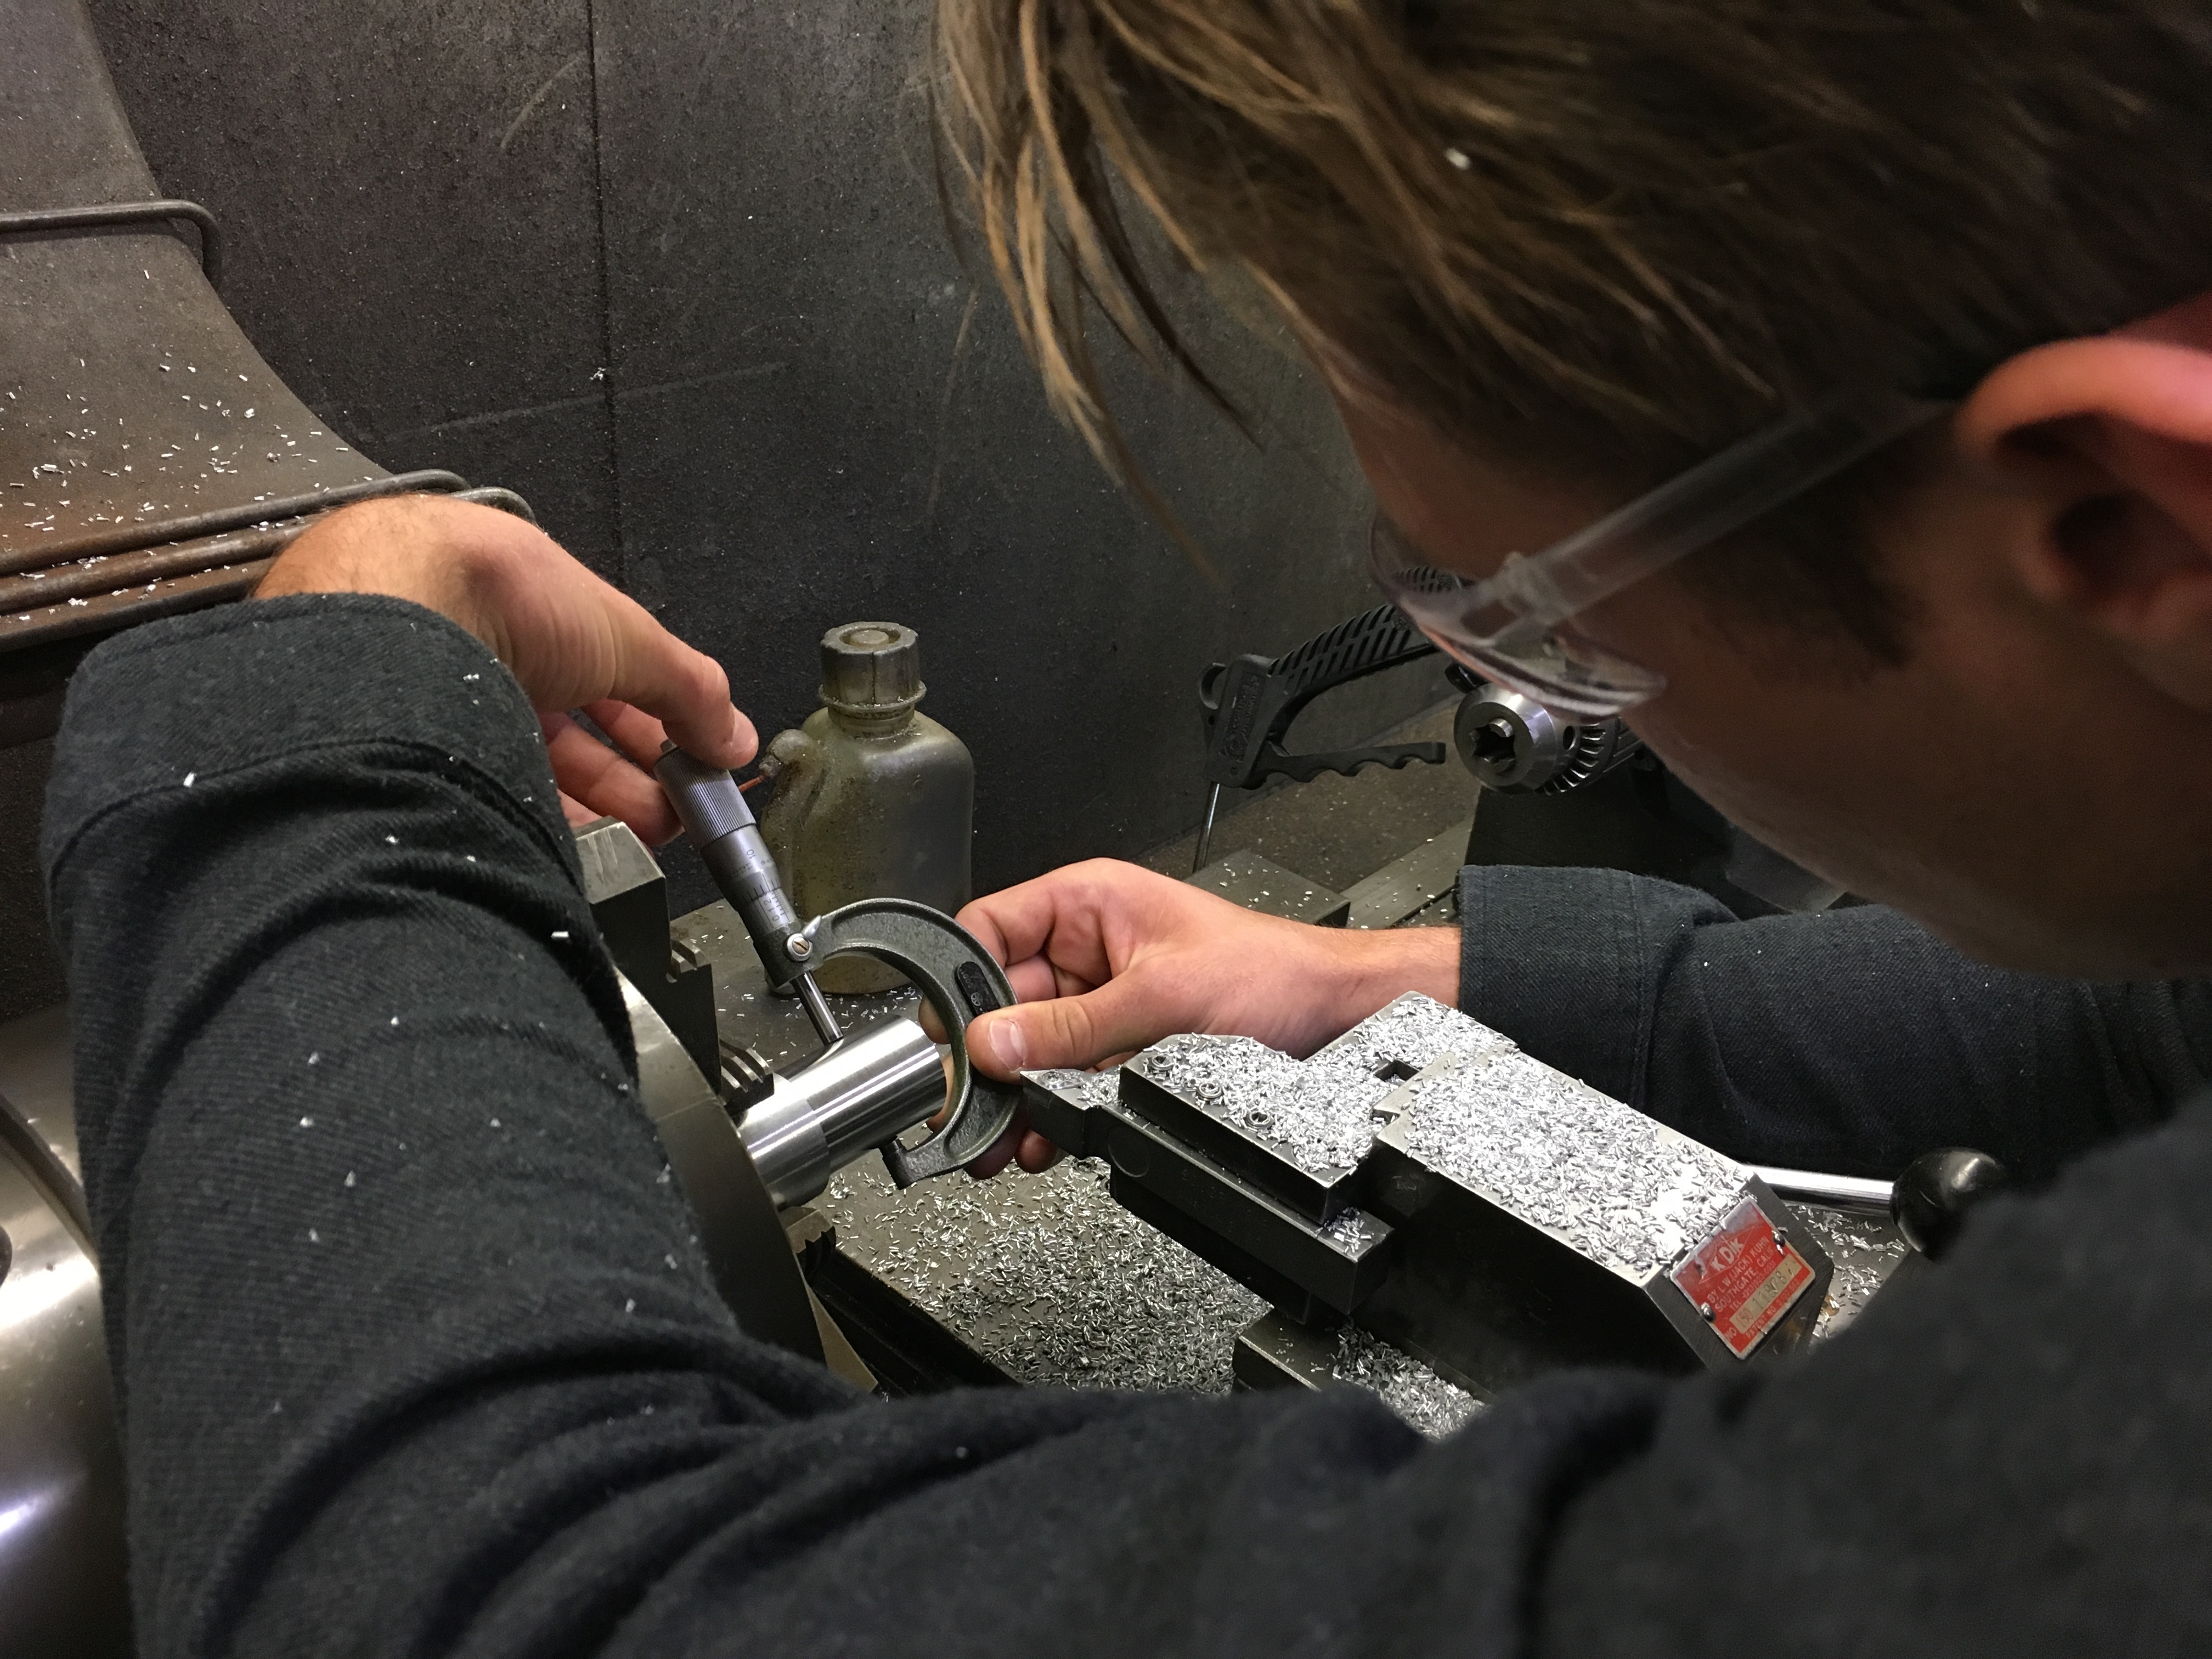
\includegraphics[width=.6 \textwidth]{08_10-22/images/IMG_0330.JPG}
    \caption{Oren checking part measurements}
    \label{fig: Turning Inserts}
\end{figure}


\end{document}